% This is the code that generates the slides we'll use for this section.
% If you'd simply like to view the slides, please open slides.pdf


\documentclass[10pt, aspectratio=169]{beamer}

\makeatletter
  \def\beamer@calltheme#1#2#3{%
    \def\beamer@themelist{#2}
    \@for\beamer@themename:=\beamer@themelist\do
    {\usepackage[{#1}]{\beamer@themelocation/#3\beamer@themename}}}

  \def\usefolder#1{
    \def\beamer@themelocation{#1}
  }
  \def\beamer@themelocation{}

\usefolder{../__resources__/beamer_theme}
\usetheme{nathan}

\addtobeamertemplate{navigation symbols}{}{%
    \usebeamerfont{footline}%
    \usebeamercolor[fg]{footline}%
    \hfill%
    \insertframenumber/\inserttotalframenumber
}

\title{Computational Decision Making for Regular People}
\subtitle{03: Math Modeling With Pyomo}
\date{October 29, 2024}

\usepackage[font=tiny,labelfont=bf]{caption}
\usepackage{caption}
\captionsetup[figure]{labelformat=empty}

\usepackage{listings}
\usepackage{dirtree}

\begin{document}

\begin{frame}
    \maketitle
\end{frame}

\begin{frame}{Today's Outline}
    \begin{columns}
        \begin{column}{0.5\textwidth}
            \begin{enumerate}
                \item Refresher on Math Modeling (Route Planning Problem)
                \item Introduction to Pyomo
                \begin{itemize}
                    \item The Pyomo "ConcreteModel"
                    \item Sets
                    \item Parameters
                    \item Variables
                    \item Constraints
                    \item Objectives
                    \item Solvers
                \end{itemize}
                \item Coding and Solving the Route Planning Problem
                \item Plotting / Exporting Results
                \item My Recommended Pyomo Workflow
                
                (The Single Responsibility Principle)
                \item "Infeasible", "Unbounded" ?
            \end{enumerate}
        \end{column}
        \begin{column}{0.5\textwidth}
            \begin{figure}
                \begin{figure}
                    
\includegraphics[width=0.95\linewidth]{PyomoLogo.png}
                \end{figure}
            \end{figure}
        \end{column}
    \end{columns}
\end{frame}

\begin{frame}{Refresher on Math Modeling}
    \textit{Given the roads indicated in the graph below, what's the fastest way to get from point A to point D?}

    \vspace{1.0cm}
    
    \begin{columns}
        \begin{column}{0.5\textwidth}
            \begin{enumerate}
                \item Objective Function ($f(\overline{X}$))
                \item Decision Variables ($\overline{X}$)
                \item Parameters ($\overline{\alpha}$)
                \item Constraints ($\textbf{S}$)
            \end{enumerate}
        \end{column}
        \begin{column}{0.5\textwidth}
            \begin{figure}
                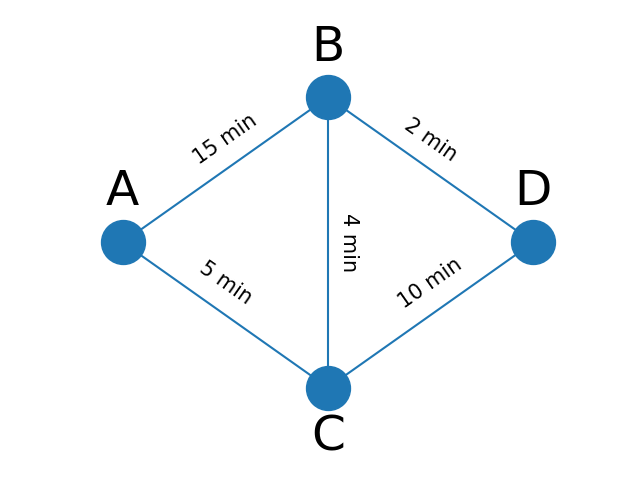
\includegraphics[width=\linewidth]{../01_Introduction/RoutePlanningProblem.png}
            \end{figure}
        \end{column}
    \end{columns}
\end{frame}

\begin{frame}{Refresher on Math Modeling}
    $$---\text{ FULL FORMULATION }---$$
    $$\min_{X_r,Y_p} \sum_{r \in \textbf{R}} \delta_r X_r$$
    $$s.t.\ \ \ \sum_{r \in \textbf{R}_p} X_r = 2 Y_p \ \ \ \forall p \in \textbf{P}^{NON-TERM}$$
    $$\sum_{r \in \textbf{R}_p} X_r = Y_p \ \ \ \forall p \in \textbf{P}^{TERM}$$
    $$Y_p = 1 \ \ \ \forall p \in \textbf{P}^{TERM}$$
    $$X_r, Y_p \in \{0,1\}$$
\end{frame}

\begin{frame}{Introduction to Pyomo}
    \begin{center}
        \textit{Before we jump in, please open up the Jupyter Notebook for today:}
    
        \textit{03\_MathematicalModelingWithPyomo/Lecture\_03\_Notebook.ipynb}
    \end{center}

    \begin{itemize}
        \item "Pyomo" Stands for "Python Optimization Modeling Objects"
        \item It is a collection of custom data structures ("modeling objects") that help organize mathematical models in Python.
        \item The most important strucutres we'll deal with are as follows:
        \begin{itemize}
            \item ConcreteModel
            \item Sets
            \item Parameters
            \item Variables
            \item Constraints
            \item Objectives
            \item Solvers
        \end{itemize}
        \item Notice now, and as we move forward, how these data structures line up with the mathematical model elements we've talked about.
        \item We'll go over each data structure in detail.
    \end{itemize}
\end{frame}

\begin{frame}{Pyomo: ConcreteModel}
    \begin{itemize}
        \item In Pyomo, everything pertaining to one mathematical model is contained in one "ConcreteModel" object.
        \item In your Python code, this will often be called "model" and will be defined something like this:
        
        \hspace{0.25cm} import pyomo.environ as pyo

        \vspace{0.25cm}
        
        \hspace{0.25cm} model = pyo.ConcreteModel()

        \item You can think of the "model" object as the home for everything pertaining to your mathematical model: All sets, variables, constraints, objectives, etc. will live inside one model object.
    \end{itemize}
\end{frame}

\begin{frame}{Pyomo: Sets}
    \begin{itemize}
        \item Recall in Lecture 01 how we used sets to reduce the amount of equations we wrote.
        \item We simply defined a set and then indicated that a certain Variable, Constraint, etc. should be repeated for every element in that set.
        \item Pyomo has a "Set" object. This is different than a built-in Python set boject.
        \item Pyomo "Set" objects have some special abilities such as the ability to multiply two sets together to make a new set of all combinations of the original two sets.
        \item Pyomo "Set" objects are defined like this:
        
        \hspace{0.25cm} model.mySet = pyo.Set(initialize=[\_\_elements\_\_])

        \item Notice how "mySet" is defined as part of the "model" object.
        \item Example: See Jupyter Notebook
    \end{itemize}

    \begin{center}
        $\textbf{R} \rightarrow $ model.R = pyo.Set(initialize=[...])
    \end{center}
\end{frame}

\begin{frame}{Pyomo: Parameters}
    \begin{itemize}
        \item Recall from Lecture 01 that parameters are simply pre-specified constant numbers.
        \item Pyomo does not have an explicit representation of these parameters.
        \item Instead, the value of each parameter is stored and communicated to Pyomo using regular Python variables.
        \item Examples: See Jupyter Notebook
    \end{itemize}
    \begin{center}
        $\delta_r \rightarrow $ delta = \{"AB": 15, "AC": 5, "BC": 4, ...\}
    \end{center}
\end{frame}

\begin{frame}{Pyomo: Variables}
    \begin{itemize}
        \item Recall in Lecture 01 how we define decision variables over a set and a domain:
        $$X_r \ \ \forall r \in \textbf{R} \left(\textbf{Binary\ Variable}\right)$$
        \item Pyomo has a "Var" object that represents a decision variable.
        \item Pyomo "Var" objects are defined like this:
        
        \hspace{0.25cm} model.myVar = pyo.Var(model.mySet,domain=pyo.myDomain)
        \item Notice how "myVar" is defined as part of the "model" object.
        \item Typical domains are: pyo.Binary, pyo.Reals, pyo.Integers, pyo.NonNegativeReals, etc.
        \item To access an individual element within a variable that is defined over a set, use a similar bracket notation used for Python Lists:
        
        \hspace{0.25cm} model.myVar[myIndex]

        \item Example: See Jupyter Notebook
    \end{itemize}
    \begin{center}
        $$X_r \ \ \forall r \in \textbf{R} \left(\textbf{Binary\ Variable}\right) \rightarrow $$ model.X = pyo.Var(model.R,domain=pyo.Binary)
    \end{center}
\end{frame}

\begin{frame}{Pyomo: Constraints}
    \begin{itemize}
        \item Recall in Lecture 01 how we define constraints over a set:
        $$\text{Some\ Relationship} \ \ \ \forall r \in \textbf{R}$$
        \item Pyomo has a "Constraint" object that represents each constraint.
        \item Pyomo "Constraint" objects take a little bit more setup in order to define.
        \begin{enumerate}
            \item Define a Python function that takes in the following things are arguments: the "model" object, an individual element (or combination of elements) within the set (or combination of sets) of which this constraint is to be defined.
            \item This function should return a relation between different algebraic expressions using Python's built-in relation syntax (==, \textless=, or \textgreater=)
            \item The "Constraint" object can then be defined like this:
            
            \hspace{0.25cm} model.myConstr = pyo.Constraint(model.mySet,rule=myFunction)

            \item Pyomo will then call the function ("myFunction") again and again for each element in the set ("mySet") and store the resulting relation in the constraint object ("myConstr").
        \end{enumerate}
        \item Example: See Jupyter Notebook
    \end{itemize}
\end{frame}

\begin{frame}{Pyomo: Objective}
    \begin{itemize}
        \item Recall in Lecture 01 that an objective is 1) a mathematical expression, 2) an indication of which decision variables to vary, and 3) an associated "max" or "min" keyword:
        
        $$\max_{X_r,Y_p} \sum_{r \in \textbf{R}}\delta_r X_r$$

        \item Pyomo has an "Objective" object that represents this objective.
        \item Pyomo "Objective" objects are defined like this:
        
        \hspace{0.25cm} model.myObj = pyo.Objective(expr=myExpression,sense=pyo.mySense)
    
        \item Note that since there are often lots of decision variables you want to vary, Pyomo assumes you want to vary all of the decision variables that you've defined using model.myVar = pyo.Var(...). Because of that you do not need to re-mention them here.
        \item Here "mySense" is just "maximize" or "minimize" depending on what you want to do.
        \item As with all Pyomo objects, notice how "myObj" is defined as part of the "model" object.
        \item Example: See Jupyter Notebook
    \end{itemize}

    \begin{center}
        $\max_{X_r,Y_p} \sum_{r \in \textbf{R}}\delta_r X_r \rightarrow$ 
        
        model.myObj = pyo.Objective(expr=sum(delta[r] * model.X[r] for r in model.R),sense=pyo.maximize) 
    \end{center}
\end{frame}

\begin{frame}{Pyomo: Solver}
    \begin{itemize}
        \item Now that we have our mathematical model defined, we need some way to solve it.
        \item Lots of really smart mathematicians have come up with clever algorithms to solve these problems.
        \item Pyomo developers have coded these algorithms into "solvers" for us to use.
        \item Some solvers are used by professionals to game the stock market, manage the electrical grid, etc. Those solvers can be very expensive.
        \item Other solvers are free (but considerably slower). Those solvers should be suitable for what we'll do in this class.
        \item Each solver is limited to a certain style of problem: Linear, Quadratic, Mixed-Integer (Binary), Generic Nonlinear, etc.
        \item Most of the problems we'll do in this class are "Mixed-Integer Linear" or "Mixed-Integer Non-Linear". So we'll use the free "SCIP"\footnote{https://www.scipopt.org/} solver for what we do in this class.
        \item If you followed the instructions at the end of Lecture 2, the SCIP solver should already be installed. If not, please visit https://www.scipopt.org/index.php\#download
    \end{itemize}
\end{frame}

\begin{frame}{Pyomo: Solver}
    \begin{itemize}
        \item In Pyomo, the solver object exists independently from the ConcreteModel object.
        \item Ideologically speaking, a solver acts on a model to find an optimal solution.
        \item A Pyomo solver must first be created:
        
        \hspace{0.25cm} solver = pyo.SolverFactory("scip")

        \item The main argument to the SolverFactory function is the name of the solver. If you want to switch between solvers, all you need to do is type the name of a different solver here.
        \item Once a solver object has been created, it can act on a given model using the "solver.solve" function:
        
        \hspace{0.25cm} solver.solve(model,tee=True)

        \item There are a lot of different arguments you could pass to the solver.solve function to do a variety of things:
        \begin{itemize}
            \item Print out updates about the solver's progress (tee=True)
            \item Set a time limit for the solver
            \item Set a threshold of acceptable accuracy of the optimal solution
            \item Specify advanced solver settings
            \item etc.
        \end{itemize}
        \item But these additional arguments change depending on which solver you're using and can get pretty complicated. So we'll just use "tee=True".
    \end{itemize}
\end{frame}

\begin{frame}{Pyomo: Accessing Results}
    \begin{itemize}
        \item Once the solver.solve function has been executed, assuming the solver was able to find a solution, the solution will be stored within the ConcreteModel itself.
        \item You can evaluate the value of any variable or expression using the "pyo.value" function.
        \begin{itemize}
            \item myVarValue = pyo.value(model.myVar[myIndex])
            \item myExpressionValue = pyo.value(model.myVar[myIndex1] + model.myVar[myIndex2])
        \end{itemize}
        \item These results can then be plotted, saved to an excel file, etc. (See Lecture 02)
    \end{itemize}
\end{frame}

\begin{frame}{Full-Blown Example Problem}
    \begin{center}
        We'll solve the Route Planning Problem we've been discussing.

        \vspace{1 cm}

        Please open up the Jupyter Notebook for Lecture 03.
    \end{center}
    
\end{frame}

\begin{frame}{The Single Responsibility Principle}
    \begin{center}
        There is a notion in the world of software developers that

        \textbf{Every function, script, data structure, etc. should have one single Responsibility.}
    \end{center}
    \begin{itemize}
        \item There are a lot of things to go on in constructing, solving, and interpreting mathematical models.
        \item Having them all jammed into one Python script can make your code hard to read and more prone to errors.
        \item I highly recommend breaking each part of this process into it's own function or script.
        \item One huge advantage of doing this is that if, down the road, you need to run just a small potion of your code, you can just call that one function or script instead of re-running the whole thing or trying to copy and paste pieces of your code that might not work if taken out of context.
    \end{itemize}
\end{frame}

\begin{frame}{My Recommended Pyomo Workflow}
    \begin{itemize}
        \item In order to make my code clean and easy to read, I break up my code like this:
        \begin{itemize}
            \item \textbf{Parameters Class}: First define a custom data type (a.k.a. Class) called "Parameters" that houses all the parameters needed to assemble an instance of a model.
            \item \textbf{AssembleModel Function}: Next define a function called "AssembleModel" that takes in a Parameters object and assembles a Pyomo ConcreteModel object equipped with all sets, variables, constraints, and objective defined. It should then return this model object.
            \item \textbf{ExecuteOptimization Function}: Next define a function called "ExecuteOptimization" that takes in a fully assembled Pyomo ConcreteModel object and executes the optimization of this model (e.g. creates a Solver object and calls solver.solve)
            \item \textbf{ExtractResults Function}: Next define a function called "ExtractResults" that takes in a full assembled and optimized Pyomo ConcreteModel object and extracts the results from that object to a format you'd like (generally excel or a plot).
            \item \textbf{Main Function}: Finally, define a function called "main" that takes no arguments but first defines a Parameters object, uses this Parameters object to assemble a Pyomo Model (using AssembleModel). Then pass this assembled model to ExecuteOptimization, and extract the results using ExtractResults.
        \end{itemize}
        \item Let's see how this looks for the Route Planning model we've already made (See Jupyter Notebook).
    \end{itemize}
\end{frame}

\begin{frame}{Infeasible? Unbounded?}
    \begin{columns}
        \begin{column}{0.5\textwidth}
            \begin{itemize}
                \item Infeasible: There are no solutions that can satisfy all of the constraints you have in your model
                \begin{itemize}
                    \item Try temporarily removing constraints (one-by-one) to try to find the one that is causing problems. That's a good place to start looking...
                \end{itemize}
                \item Unbounded: The solver says you can keeping traveling forever in the direction indicated by your objective. Thus your optimal objective function value will be infinity.
                \begin{itemize}
                    \item Try adding bounding constraints on your variables (e.g. $X <= 1,000,000$) to make the problem bounded again. Then look at the new solution to see which variable is becoming so large. That's a good place to start looking...
                \end{itemize}
            \end{itemize}
        \end{column}
        \begin{column}{0.5 \textwidth}
            \vspace{-0.5cm}
            \begin{figure}
                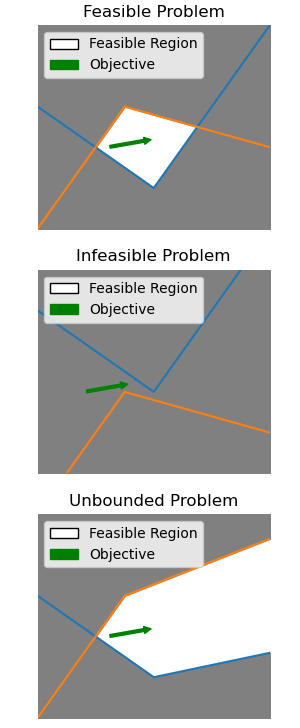
\includegraphics[width=0.4\linewidth]{InfeasibleUnbounded.png}
            \end{figure}
        \end{column}
    \end{columns}

\end{frame}

\begin{frame}{Next Class: Patterns in Formulations}
    \begin{itemize}
        \item In the next class we'll tackle how to represent certain real-world behaviors in mathematical models.
        \begin{itemize}
            \item How can I neatly optimize over a series of time periods, accounts, options, or all of them all at once?
            \item How can I handle uncertainty in my model parameters?
            \item What if I want different parameters to be selected if I make a certain decision?
            \item How can I handle "nonlinear" behaviors like "min", "max", and binary activation in a (mixed-integer) linear way? (I want my models to not take forever to solve)
        \end{itemize}
    \end{itemize}
\end{frame}

\end{document}